\documentclass{article}
\usepackage[a4paper,left=3cm,right=3cm,top=3cm,bottom=3cm]{geometry}
\usepackage[utf8]{inputenc}
\usepackage[T1]{fontenc}
\usepackage{latexsym,amsfonts,amsmath,amssymb,amstext,graphicx,titlesec,ae,aecompl,mathtools,tabularx, multirow, cancel, nicefrac,subcaption, blindtext, floatrow}
\setlength{\parindent}{0pt}
\newfloatcommand{capbtabbox}{table}[][\FBwidth]


\begin{document}

\begin{titlepage}
       \begin{center}
             \begin{huge}
				   %% Update assignment number here
                   \textbf{Assignment 2}
             \end{huge}
       \end{center}

       \begin{center}
             \begin{large}
                   Computational Intelligence, SS2020
             \end{large}
       \end{center}

       \begin{center}
 \begin{tabularx}{\textwidth}{|>{\hsize=.33\hsize}X|>{\hsize=.33\hsize}X|>{\hsize=.33\hsize}X|} 

                   \hline
                   \multicolumn{3}{|c|}{\textbf{Team Members}} \\
                   \hline
                   Last name & First name & Matriculation Number \\
                   \hline
                   Blöcher & Christian & 01573246 \\
                   \hline
                   Bürgener & Max & 01531577 \\
                   \hline
                    &  &  \\
                   \hline

             \end{tabularx}
       \end{center}
\end{titlepage}

\section{Linear regression}

\subsection{Derivation of Regularized Linear Regression}

%\begin{itemize}

%    \begin{figure}[h]
%        \centering
%        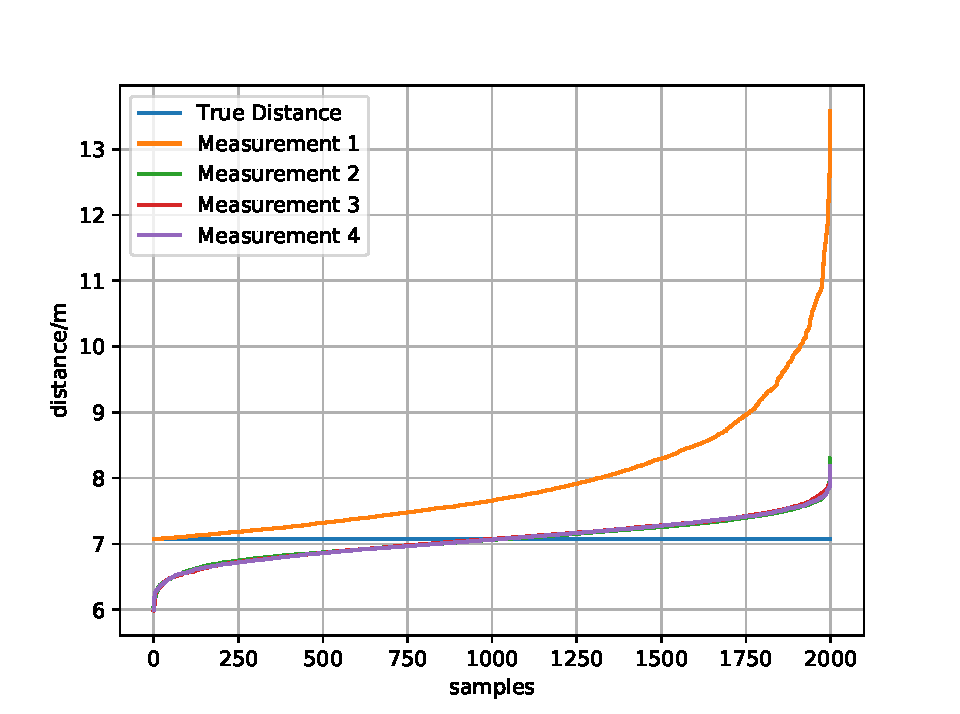
\includegraphics[width=\textwidth]{./Figures/scenario2_findexponential.pdf}
%        \caption{Scenario 2 with mixed measurement models for the anchors}
%        \label{fig:scenario2_findexponential}
%    \end{figure}
    
%    \item In figure \ref{fig:scenario2_findexponential} we can see that in scenario 2 the distance measurements from anchor 1 is exponentially distributed. It is the only distribution which is bigger than the true distance for all samples and its slope is rising exponentially for rising x-values.
    
%\end{itemize}

\subsection{Linear Regression with polynomial features}

\begin{itemize}

    \item Analytical derivation for the Gaussian distribution:\\
  
	    $\begin{array}{ccc}
	        p(\tilde{d}_n(a_i,\mathbf{p})\mid\mathbf{p}) & = & \frac{1}{\sqrt{2\pi\sigma^2}} \cdot e^{- \frac{[\tilde{d}_n(a_i,\mathbf{p})-d(a_i,\mathbf{p})]^2}{2\sigma^2}} \\  
	    \end{array}$\\
	    
	    The data is independent identically distributed (iid), therefore the likelihood function is the product of all individual likelihoods\\
	    
	    $\begin{array}{ccc}
	        P(\tilde{d}_n(a_i,\mathbf{p})\mid\mathbf{p}) & = & \displaystyle \prod_{n=0}^{N-1} \frac{1}{\sqrt{2\pi\sigma^2}} \cdot e^{- \frac{[\tilde{d}_n(a_i,\mathbf{p})-d(a_i,\mathbf{p})]^2}{2\sigma^2}} \\

	    \end{array}$\\
	  
	    To convert the product to a sum we apply the natural logarithm.\\
	  
	    $\begin{array}{cccl}
	        L(\tilde{d}_n(a_i,\mathbf{p})\mid\mathbf{p}) & = & ln \left[ \displaystyle \displaystyle \prod_{n=0}^{N-1} \frac{1}{\sqrt{2\pi\sigma^2}} \cdot e^{- \frac{[\tilde{d}_n(a_i,\mathbf{p})-d(a_i,\mathbf{p})]^2}{2\sigma^2}} \right] & \\\\
	        L(\tilde{d}_n(a_i,\mathbf{p})\mid\mathbf{p}) & = & \displaystyle \sum_{n=0}^{N-1} \left[ ln(\frac{1}{\sqrt{2\pi\sigma^2}}) - \frac{[\tilde{d}_n(a_i,\mathbf{p})-d(a_i,\mathbf{p})]^2}{2\sigma^2} \right] & \\
	    \end{array}$\\
	  
	    Since we want to find the parameter $\sigma^2$, which maximizes the probability of the distance, we derive $L(\tilde{d}_n(a_i,\mathbf{p})\mid\mathbf{p})$ and set it to zero. \\
	
	    $\begin{array}{cccr}
	        L(\tilde{d}_n(a_i,\mathbf{p})\mid\mathbf{p}) & = & \displaystyle \sum_{n=0}^{N-1} \left[ ln(1) - \frac{1}{2}ln(2\pi\sigma^2) - \frac{[\tilde{d}_n(a_i,\mathbf{p})-d(a_i,\mathbf{p})]^2}{2\sigma^2} \right] & \mid \frac{\partial}{\partial\sigma^2} \\\\
	        \frac{\partial}{\partial\sigma^2} L(\tilde{d}_n(a_i,\mathbf{p})\mid\mathbf{p}) & = & \displaystyle \sum_{n=0}^{N-1} \left[ - \frac{1}{\sigma^2} + \frac{[\tilde{d}_n(a_i,\mathbf{p})-d(a_i,\mathbf{p})]^2}{\sigma^4} \right] & \stackrel{!}{=} 0 \\\\
	        0 & = & \displaystyle \sum_{n=0}^{N-1} \left[ - \frac{1}{\sigma^2} + \frac{[\tilde{d}_n(a_i,\mathbf{p})-d(a_i,\mathbf{p})]^2}{\sigma^4} \right] & \\\\
	        \frac{N}{\sigma^2} & = & \displaystyle \sum_{n=0}^{N-1} \frac{[\tilde{d}_n(a_i,\mathbf{p})-d(a_i,\mathbf{p})]^2}{\sigma^4} \\\\
	        \sigma^2 & = & \frac{\displaystyle \sum_{n=0}^{N-1}[\tilde{d}_n(a_i,\mathbf{p})-d(a_i,\mathbf{p})]^2}{N} 
	    \end{array}$\\
         	 
	\item Analytical derivation for the Exponential distribution:\\
	 
	    \begin{equation*}
	  	     p(\tilde{d}_n(a_i,\mathbf{p})\mid\mathbf{p}) = 
	         \begin{cases}
	             \lambda_i e^{-\lambda_i [\tilde{d}_n(a_i,\mathbf{p}) - d(a_i,p)]} & \quad \text{, }\tilde{d}_n(a_i,\mathbf{p}) \geq d(a_i,\mathbf{p}) \\
	             0 & \quad \text{, else}
	         \end{cases}
	     \end{equation*}
	    
            	         
	     $\begin{array}{cccl}
	         L(\tilde{d}_n(a_i,\mathbf{p}) \mid \mathbf{p}) & = & \displaystyle \sum_{n=0}^{N-1} ln(\lambda_i) - \lambda_i [\tilde{d}_n(a_i,\mathbf{p}) - d(a_i,\mathbf{p})] & \mid \frac{\partial}{\partial\lambda_i} \\\\
	         \frac{\partial}{\partial\lambda_i} L(\tilde{d}_n(a_i,\mathbf{p}) \mid \mathbf{p}) & = & \frac{N}{\lambda_i} - \displaystyle \sum_{n=0}^{N-1}[\tilde{d}_n(a_i,\mathbf{p}) - d(a_i,\mathbf{p})] & \stackrel{!}{=} 0 \\\\
	         \frac{N}{\lambda_i} & = & \displaystyle \sum_{n=0}^{N-1} [\tilde{d}_n(a_i,\mathbf{p}) - d(a_i,\mathbf{p})] & \\\\
	         \lambda_i & = & \frac{N}{\displaystyle \sum_{n=0}^{N-1} [\tilde{d}_n(a_i,\mathbf{p}) - d(a_i,\mathbf{p})]} & ,\tilde{d}_n(a_i,\mathbf{p}) \geq d(a_i,\mathbf{p})
	     \end{array}$\\
	 
\end{itemize}

\subsection{(Bonus) Linear Regression with radial basis functions}


\section{Logistic Regression}

\subsection{Derivation of Gradient}

\begin{itemize}
    \item Analytical conversion of the ML estimation equation:\\
    
        $\begin{array}{ccccl}
        	\hat{\mathbf{p}}_{ML}(n) & = & \underset{\mathbf{p}}{\textrm{argmax}} \displaystyle \prod_{i=0}^{N_A-1} p(\tilde{d}_n(a_i,\mathbf{p})\mid\mathbf{p}) & &\\
        	\hat{\mathbf{p}}_{ML}(n) & = & \underset{\mathbf{p}}{\textrm{argmax}} \;ln \left[ \displaystyle \prod_{i=0}^{N_A-1} p(\tilde{d}_n(a_i,\mathbf{p})\mid\mathbf{p}) \right] & &\\        
        	\hat{\mathbf{p}}_{ML}(n) & = & \underset{\mathbf{p}}{\textrm{argmax}} \displaystyle \sum_{i=0}^{N_A - 1} ln \left( \frac{1}{\sqrt{2\pi\sigma_i^2}}\right) - \frac{[\tilde{d}_n(a_i,\mathbf{p})-d(a_i,\mathbf{p})]^2}{2\sigma_i^2} & &\\
        \end{array}$ \\
       
        Because in scenario 1 we only use Gaussian models for all anchors that were calibrated with the same distance to the reference position, we can assume that $\sigma_i^2 = \sigma^2 \; \forall i$. That means the $ln$-term can be neglected since it only shifts the value of the maximum by a constant but does not affect its position. Similarly $\frac{1}{2\sigma^2}$ can be omitted, as it is also just a scaling factor. Furthermore $ \underset{\mathbf{p}}{\textrm{argmax}}\;(- \dots)$ is equivalent to $\underset{\mathbf{p}}{\textrm{argmin}}\;(\dots)$. Thus: \\
        
        $\begin{array}{ccccl}
        
        	\hat{\mathbf{p}}_{ML}(n) & = & \underset{\mathbf{p}}{\textrm{argmin}} \displaystyle \sum_{i=0}^{N_A-1} [\tilde{d}_n(a_i,\mathbf{p})-d(a_i,\mathbf{p})]^2 & = & \hat{\mathbf{p}}_{LS}(n)
        	    	
        \end{array}$
                 	
\end{itemize}



\subsection{Logistic Regression training with gradient descent}

\end{document}}